\chapter[Network Theory \& Computational Methods]{Network Theory \\ \& Computational Methods}
\label{ch:methods}

This chapter discusses the theory underpinning complex networks, covering the representation of atomic systems as networks and the relationship of the dual network to ring structure.
The laws which govern the topological properties of physical networks, namely Euler's law, \lm's law and the \aw{} law are also explored.
Further developments linking to modern network science etc. are given in chapter \davidnote{Link to network theory later}.
In addition some of the existing computational approaches for generating realisations of \td{} networks are presented.
A broad overview of \mc{} methods is given, before specific methods are covered in detail.
These include the bond switching algorithm and hard particle \mc{} in conjunction with the Voronoi construction.
Extensions to these methods and additional approaches are outlined in the relevant chapters \davidnote{Link to bond switching/Voronoi/mx2/procrystals later}.
Finally some measures are discussed...

\section{Network Theory}
\label{sec:networktheory}

The scope of what constitutes a complex network is extremely broad, covering everything from the tangible (\eg{} computational clusters) to the more abstract (\eg{} social interactions). Yet part of the appeal and power of network science is the ability to quantify and relate these highly disparate systems with the same underlying theory.
A network is simply a collection of components termed \textit{nodes} and the connections between them termed \textit{links}, an example of which is given in figure \ref{fig:smallnet}.
There are then two fundamental classes of network based on the nature of the connections.
Networks in which the links between nodes are mutual are termed undirected, whereas those in which the links are one\--way are termed directed \cite{barabasi2016n}.
At the risk of dating this thesis, this is the difference between Facebook (an undirected social network of friends) and Twitter (a directed social network of followers).
All the networks considered in this work are undirected and all the theory assumes this property.

\begin{figure}[h]
     \centering
      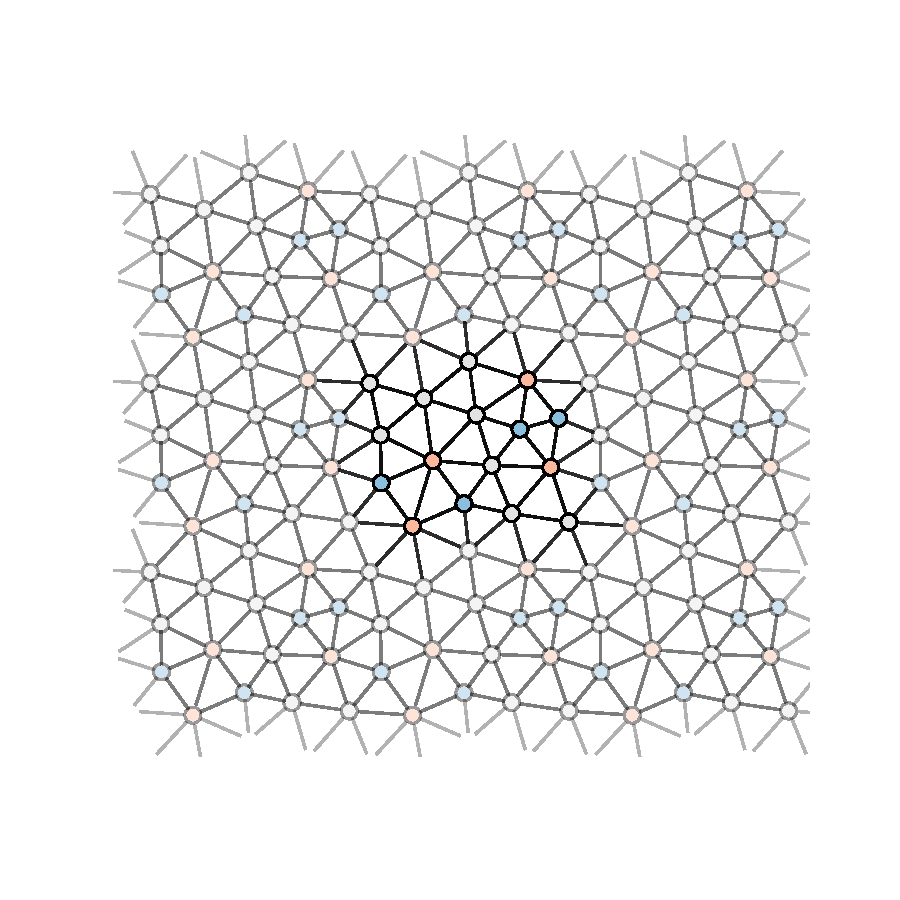
\includegraphics[width=8cm]{./figures/methods/small_periodic_net.pdf}
     \caption{Example of a periodic \td{} network where nodes are represented by circles and links as lines. Nodes are coloured similarly according to their degree, whilst periodic images are greyed out to highlight the central repeating unit.}
     \label{fig:smallnet}
\end{figure}

\subsection{Node Degree and Probability Distributions} 

A key concept in network science is the the node degree, defined as the number of links that each node possesses.
A node with $k$ links is then said simply to have degree $k$, where $k\in\mathbb{N}$.
This is illustrated in figure \ref{fig:smallnet}, which consists of 5\-- (blue), 6\-- (grey) and 7\-- (red) degree nodes.
The occurrence and correlations of nodes of given degrees can then be described by a range of probability distributions.

The probability of a randomly selected node having degree $k$ is given by the node degree distribution, denoted $p_k$.
This is a normalised discrete distribution such that
\begin{equation}
	\label{eq:pknorm}
	\sumk p_k = 1 \,.
\end{equation}
The $n$\th{} moments of this distribution are then given by:
\begin{equation}
	\label{eq:pkmoment}
	\langle k^{n} \rangle = \sumk k^np_k \,.
\end{equation}
Alternatively, one can also calculate the probability that a randomly selected link has a $k$\--degree node at the end, denoted $q_k$.
This is not the same as the distribution above, as there is greater chance of selecting links which emanate from high degree nodes, in a manner which is proportional to the node degree.
As this distribution is normalised, this leads to the relations:
\begin{align}
	\sumk q_k &= 1 \label{eq:qknorm} \\
	q_k &= \frac{kp_k}{\langle k \rangle} \label{eq:qkpk} \,.
\end{align}
In addition, one can also evaluate the probability that a randomly chosen link has nodes of degree $j$,$k$ at either end.
This is the node joint degree distribution, denoted $e_{jk}$. 
Once again this is normalised and satisfies the following relationships:
\begin{align}
	\sumjk e_{jk} &= 1, \label{eq:ejknorm} \\
	\sumjk e_{jk} &= q_j \label{eq:ejkqk} \\
	e_{jk} &= e_{kj} \label{eq:ejkekj} \,,
\end{align}
where the final result arises from reciprocal nature of the links in an undirected network.
As an example, these three probability distributions are provided for the network in figure \ref{fig:smallnet}:
\begin{align}
	\mathbf{p} =  \frac{1}{16} \, \begin{blockarray}{*{1}{c} l}
	\begin{block}{[*{1}{c}]>{$\footnotesize}l<{$}}
	4 \: \bigstrut[t]& 5\\
	8 & 6 \\
	4 & 7 \\
	\end{block}
	\end{blockarray}
	\qquad
	\mathbf{q} =  \frac{1}{96} \, \begin{blockarray}{*{1}{c} l}
	\begin{block}{[*{1}{c}]>{$\footnotesize}l<{$}}
	20 \: \bigstrut[t]& 5\\
	48 & 6 \\
	28 & 7 \\
	\end{block}
	\end{blockarray}
	\qquad	
	\mathbf{e} = \frac{1}{96}\: \begin{blockarray}{*{3}{c} l}
	\begin{block}{*{3}{>{$\footnotesize}c<{$}} l}
	5 & 6 & 7 \\
	\end{block}
	\begin{block}{[*{3}{c}]>{$\footnotesize}l<{$}}
	2 & 9 & 9 \: \bigstrut[t]& 5\\
	9 & 22 & 17 & 6 \\
	9 & 17 & 2 & 7\\
	\end{block}
	\end{blockarray} \, .
%	\textbf{p} = \frac{1}{96}\: \begin{blockarray}{*{5}{c} l}
%	\begin{block}{*{5}{>{$\footnotesize}c<{$}} l}
%	3 & 6 & 7 & 8 & 9 \\
%	\end{block}
%	\begin{block}{[*{5}{c}]>{$\footnotesize}l<{$}}
%	0 & 0 & 5 & 10 & 1\: \bigstrut[t]& \:3\\
%	0 & 0 & 1 & 1 & 0 & \:6 \\
%	5 & 1 & 14 & 14 & 1 & \:7\\
%	10 & 1 & 14 & 14 & 1 & \:8\\
%	1 & 0 & 1 & 1 & 0 & \:9\\
%	\end{block}
%	\end{blockarray}
\end{align}

\subsection{Atomic and Ring Networks}

To see how network theory relates to atomic materials, consider the amorphous graphene configuration in figure \ref{fig:graphdualgraph}.
In this network the nodes represent carbon atoms and the links sp$^2$ bonds.
The node degree in the atomic network for all nodes is then equal to three, being equivalent to the atomic coordination number (which throughout this thesis will be denoted by $c$).
This is problematic, because whilst there is clear disorder in the system, it is not well captured by the atomic network.
Due to the fact that the local environment around the atoms is identical, when examining say the node degree distribution any information about the glassy structure is lost.
This network is to first order indeterminable from a crystalline hexagonal lattice.

\begin{figure}[h]
     \centering
     
     \begin{subfigure}[b]{0.3\textwidth}
         \centering
         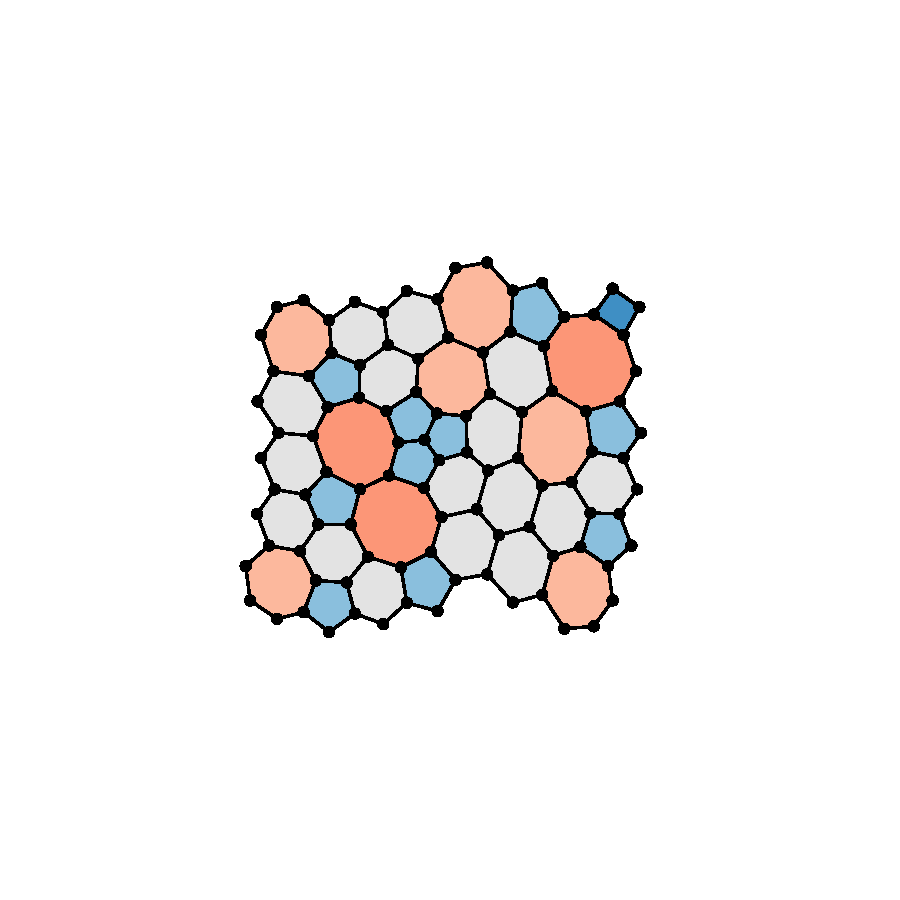
\includegraphics[width=\textwidth]{./figures/methods/graph.pdf}
         \caption{Atomic network.}
         \label{fig:graphdualgraph}
     \end{subfigure}
     \hfill
	\begin{subfigure}[b]{0.3\textwidth}
         \centering
         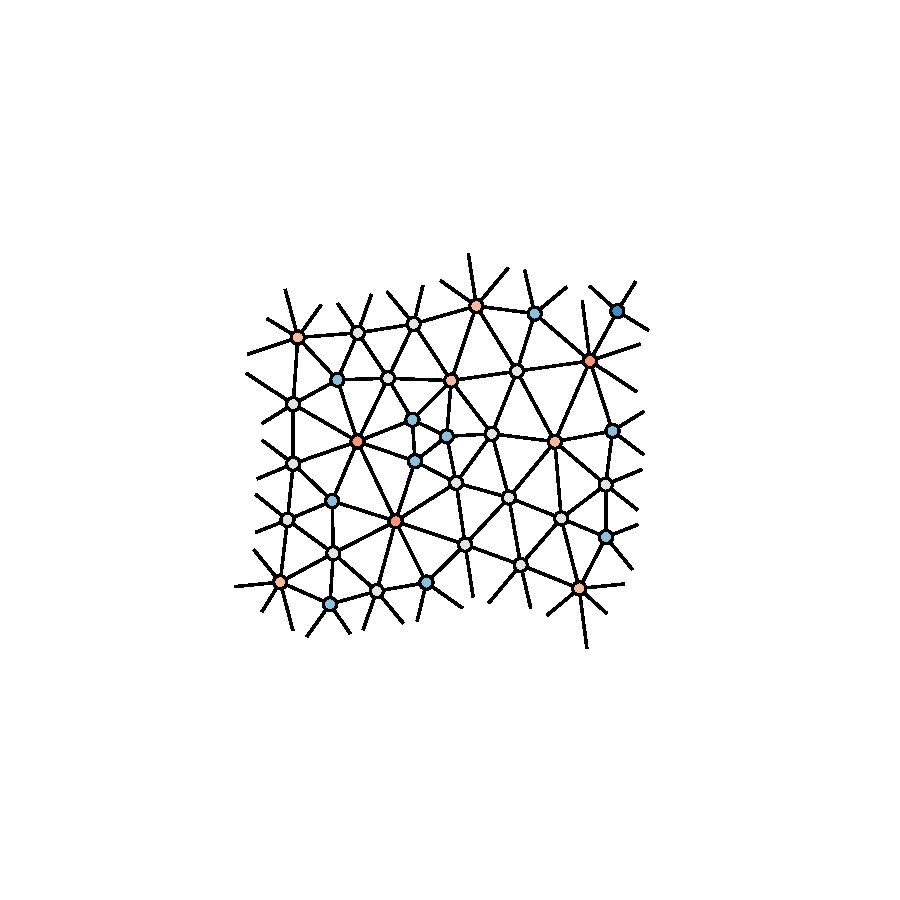
\includegraphics[width=\textwidth]{./figures/methods/dual.pdf}
         \caption{Ring network.}
         \label{fig:graphdualdual}
     \end{subfigure}
     \hfill
     \begin{subfigure}[b]{0.3\textwidth}
         \centering
         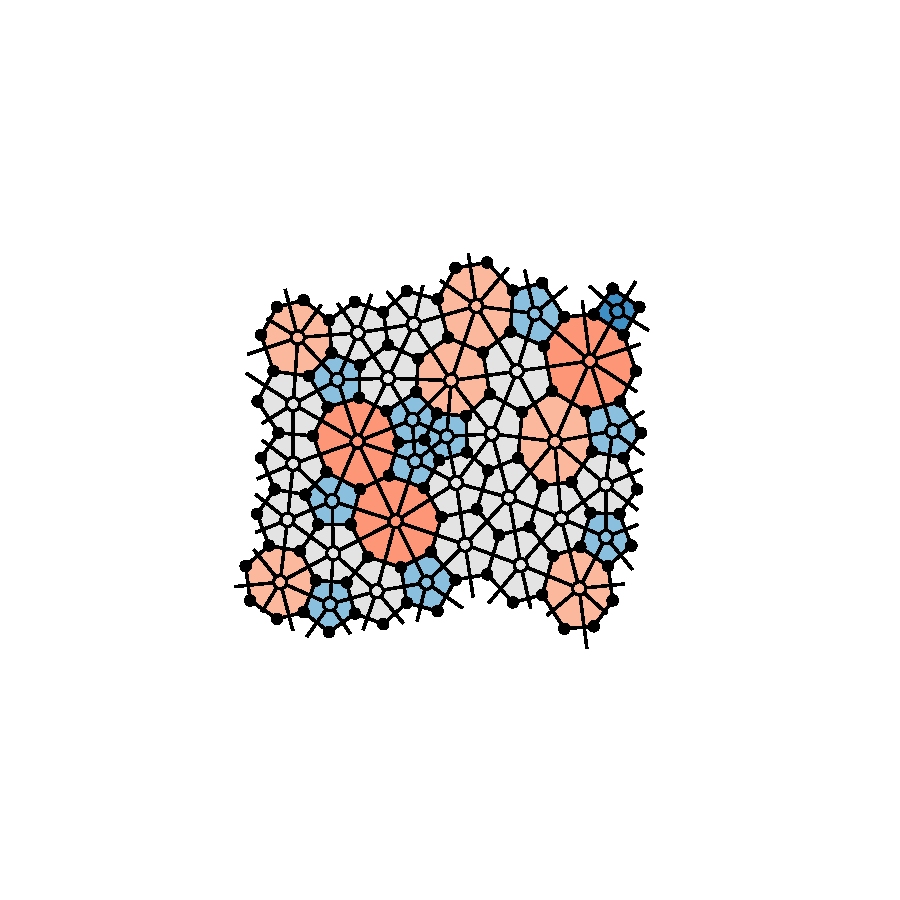
\includegraphics[width=\textwidth]{./figures/methods/graph_dual.pdf}
         \caption{Dual relationship.}
         \label{}
     \end{subfigure}
     \hfill
     
     \caption{Panel (a) gives an example of a 3\-- coordinate periodic atomic network with disordered ring structure. Nodes and links represent atoms and bonds respectively where rings are coloured by size. Panel (b) gives the corresponding ring network where nodes and links represent rings and their adjacencies, where nodes are coloured by degree. Panel (c) shows the dual relationship between the atomic and ring networks, where the node degree in the ring network is equal to the ring size in the atomic network.}
     \label{fig:graphdual}
\end{figure}

Observing figure \ref{fig:graphdualgraph} one can see there is another level of structure in the network, namely that of the ring structure.
A ring is strictly any closed path of sequentially linked nodes in a network, but this thesis will use the term in reference only to the primitive rings \ie{} those which cannot be subdivided into two smaller rings \cite{Yuan2002}.
A ring of size $k$ (or $k$\--ring) is then defined as a ring with $k$ constituent nodes.
It is clear that finding and counting the number of rings of each size, often termed calculating the ring statistics, does then quantify the disorder in the system \cite{Kumar2014}.
The ring statistics can be summarised by the normalised probability distribution, $p_k$.

However, there is a more efficient way of representing and quantifying the ring structure in the system, and that is by constructing the dual network \cite{Aboav1984}.
The dual is generated by placing a node at the centre of each ring and linking the nodes of adjacent (\ie{} edge\--sharing) rings, as can be seen in figure \ref{fig:graphdualdual}.
This will be referred to as the ring network.
The ring network is a reciprocal lattice in which the node degree, $k$, is equivalent to the ring size in the atomic network.
Similarly, it consists solely of triangles, reflecting the 3\--coordinate nature of the underlying atomic network.
Hence, the disorder is captured directly in the node properties of the ring network.
These characteristics make the ring network preferable for manipulating and analysing the systems in this thesis.

\section{Topological Laws}
\label{sec:topolaws}

There are a number of laws which govern the topological properties of \td{} network\--forming materials.
These laws constrain the ring structure, influencing the network properties in a manner that makes physical networks unique in the field of network science.
These laws act on a number of ``levels'': Euler's law controls the overall mean ring size, \lm's{} law the ring size distribution and the \aw{} law the ring\--ring correlations.

\subsection{Euler's Law}
\label{ssec:eulerslaw}

Euler's law constrains the mean ring size, $\ki$, in an atomic network or equivalently the mean node degree of the ring network.
The atomic networks studied in this work are all \td{}, connected (there is a path between any two nodes) and planar (they have no overlapping links) and so are subject to Euler's formula which states:
\begin{equation}
	\label{eq:eulerformula}
	N + V - E = \chi,
\end{equation}
where $N$, $V$, $E$ are the number of rings, vertices and edges in the network and $\chi$ in an integer termed the Euler characteristic, which is dependent on the global topology of the system.
Each vertex represents an atom and the number of edges emanating from each vertex is then the coordination number.

For generality consider an atomic network with atoms of assorted coordination numbers, $c$. 
If the proportion of each coordination type is $x_c$, then the mean coordination number is given by $\langle c \rangle = \sum\limits_c cx_c$.
This allows the number of edges to be written in terms of the number of vertices as $E=\frac{V}{2}\langle c \rangle$. 
In turn the mean ring size is simply the total number of vertices per ring, allowing for multiple counting, such that $\ki=\frac{V}{N}\langle c \rangle$.
Substituting these two expressions into equation \eqref{eq:eulerformula} leads to the expression:
\begin{equation}
	\label{eq:avdegree}
	\ki = \frac{2\langle c \rangle\left(1-\chi/N\right)}{\langle c \rangle - 2}.
\end{equation}
Hence the average node degree in the ring network (equivalent to the mean ring size of the physical network), is simply related to the average degree of the physical network (\ie{} local coordination environment), the topology of the system and the number of rings.

Although equation \eqref{eq:avdegree} may appear simple, it is a very powerful constraint. 
To demonstrate this consider a two\--dimensional lattice with two possible coordination environments $c=3,4$. 
The planar case with periodic boundary conditions (mimicking an infinite planar lattice) maps onto the torus with $\chi=0$, and so:
\begin{equation}
	\label{eq:2dplanarcases}
	\ki = \begin{cases}
		6, \quad x_3 = 1 \\
		4, \quad x_4 = 1 \\
		5, \quad x_3 = 2/3, x_4 =1/3.
	\end{cases}
\end{equation}
To reiterate in plain terms, this means that if there is a material consisting of atoms all forming exactly three bonds (as for amorphous carbon), the mean ring size \textit{must} be equal to six. 
Similarly if all atoms form four bonds the mean ring size is four, and if there is a two\--thirds to one\--third mixture of coordination environments the mean ring size is five.
The simplest illustrations of these are the hexagonal, square and cairo regular tilings, shown in figure \ref{fig:lattices}, but this law holds equally well for amorphous configurations.
For aperiodic systems strictly $\chi=1$, but as $N\rightarrow \infty$, the proportion of vertices with unsatisfied coordination on the sample perimeter become negligible overall as does the term in $\chi$.
Therefore in reality these relationships hold, and remain as applicable to amorphous graphene as the basalt columns in Fingal's Cave, and the Penrose tiling \cite{Goehring2014,Ressouche2009}.

This analysis also extends to spherical topology where $\chi=2$, and so:
 \begin{equation}
	\ki = \begin{cases}
		\frac{6N-12}{N}, \quad x_3 = 1 \\
		\frac{4N-8}{N}, \quad x_4 = 1.
	\end{cases}
\end{equation}
These relationships are the origin of the 12 pentagon rule for 3-coordinate fullerenes (the ``football problem''), or equivalently an ``8 triangle rule'' in the 4-coordinate case, as this is the only way to satisfy these equations if the allowed ring sizes are limited to $k=5,6$ and $k=3,4$ respectively (as in figures \ref{fig:latticesfull92},\ref{fig:latticesfull98}) \cite{Fowler1996}.
Much of the richness in the behaviour of \td{} physical networks stems from this fundamental constraint on the network average degree.

\begin{figure}[h]
     \centering
     
     \begin{subfigure}[b]{0.3\textwidth}
         \centering
         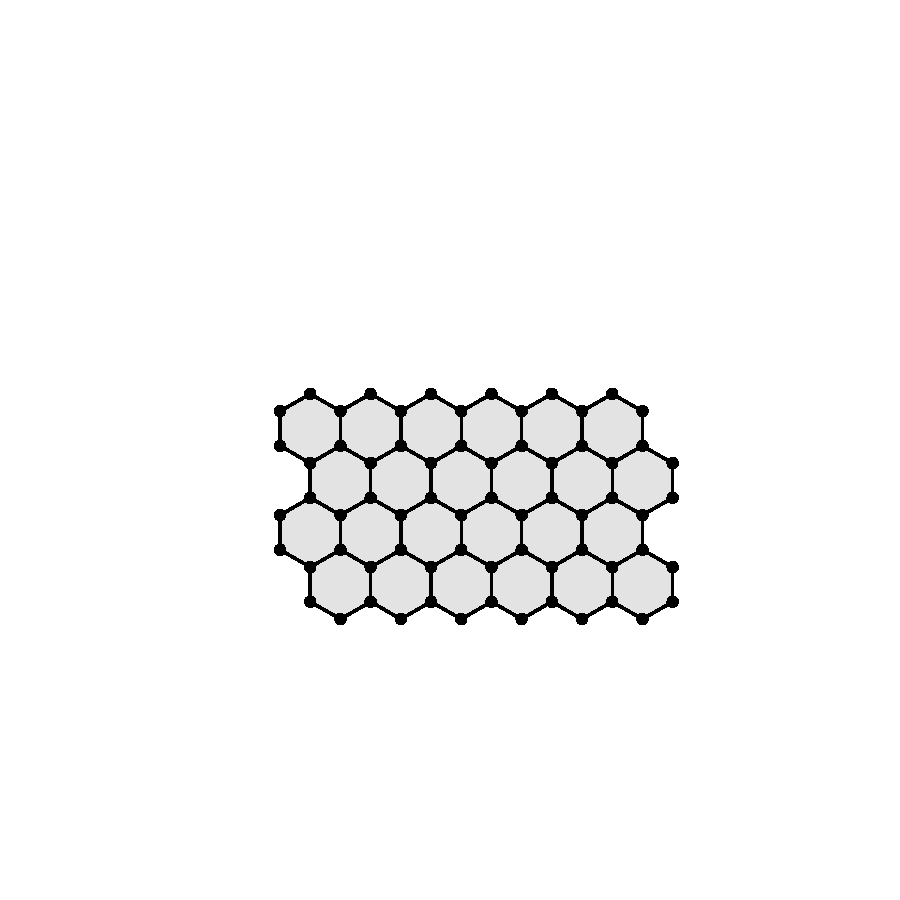
\includegraphics[height=2.4cm]{./figures/methods/hex.pdf}
         \caption{Hexagonal.}
         \label{fig:latticeshex}
     \end{subfigure}
     \hfill
     \begin{subfigure}[b]{0.3\textwidth}
         \centering
         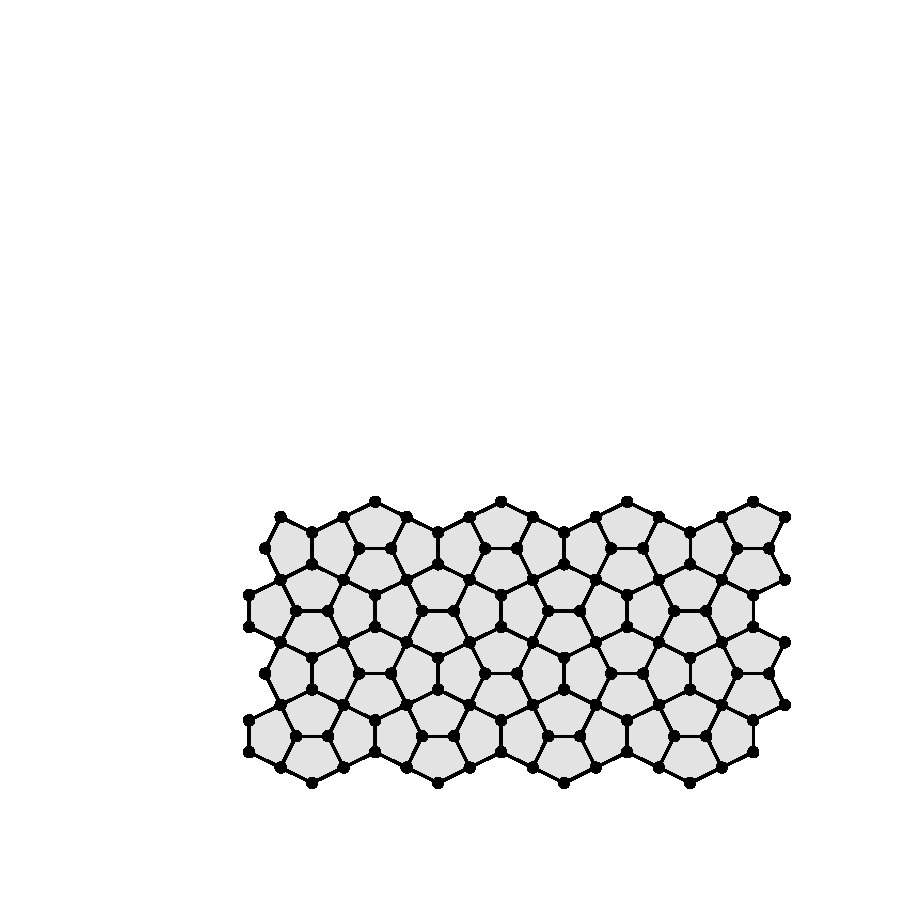
\includegraphics[height=2.4cm]{./figures/methods/cai.pdf}
         \caption{Cairo.}
         \label{fig:latticescairo}
     \end{subfigure}
     \hfill
	\begin{subfigure}[b]{0.3\textwidth}
         \centering
         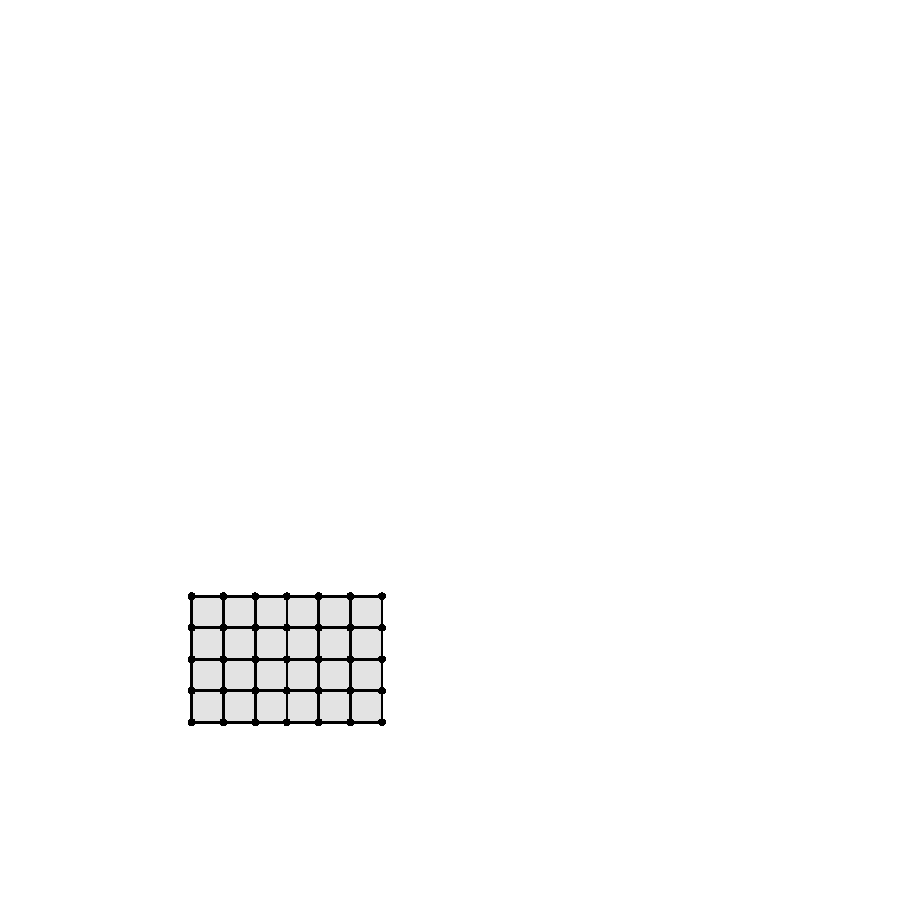
\includegraphics[height=2.4cm]{./figures/methods/sq.pdf}
         \caption{Square.}
         \label{fig:latticessq}
     \end{subfigure}
     \hfill
     \vspace{0.5cm}
     
       \begin{subfigure}[b]{0.45\textwidth}
         \centering
         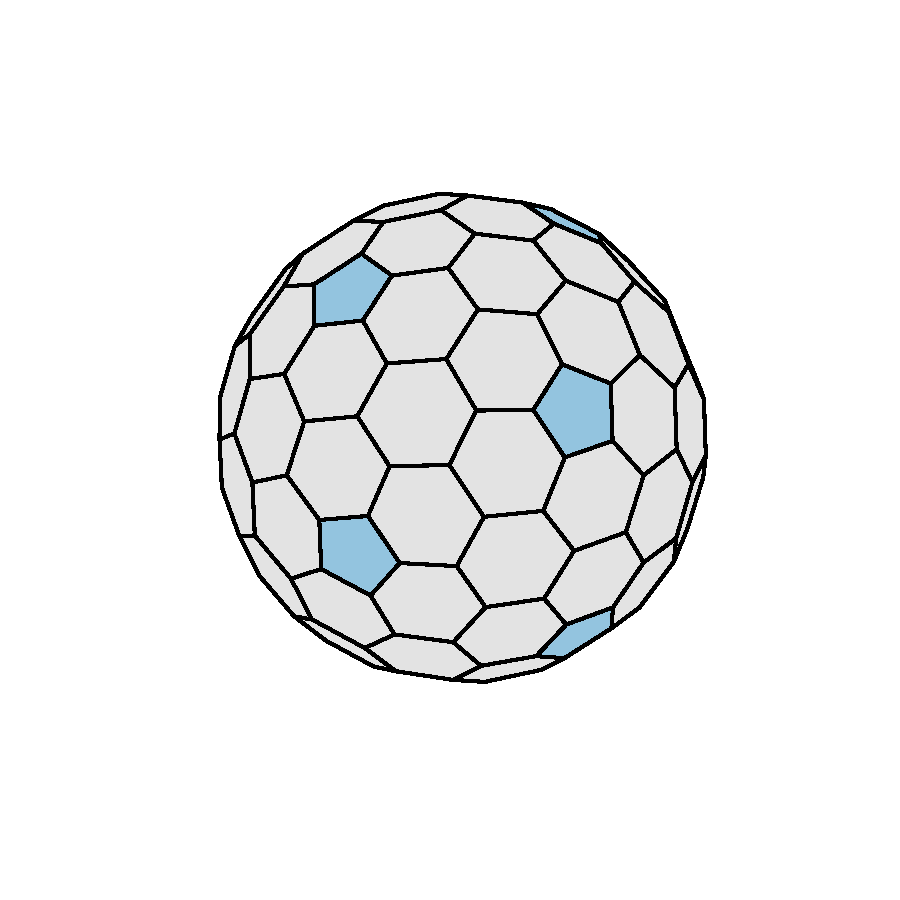
\includegraphics[height=2.4cm]{./figures/methods/full92.pdf}
         \caption{3\--coordinate fullerene.}
         \label{fig:latticesfull92}
     \end{subfigure}
     \hspace{1cm}
     \begin{subfigure}[b]{0.45\textwidth}
         \centering
         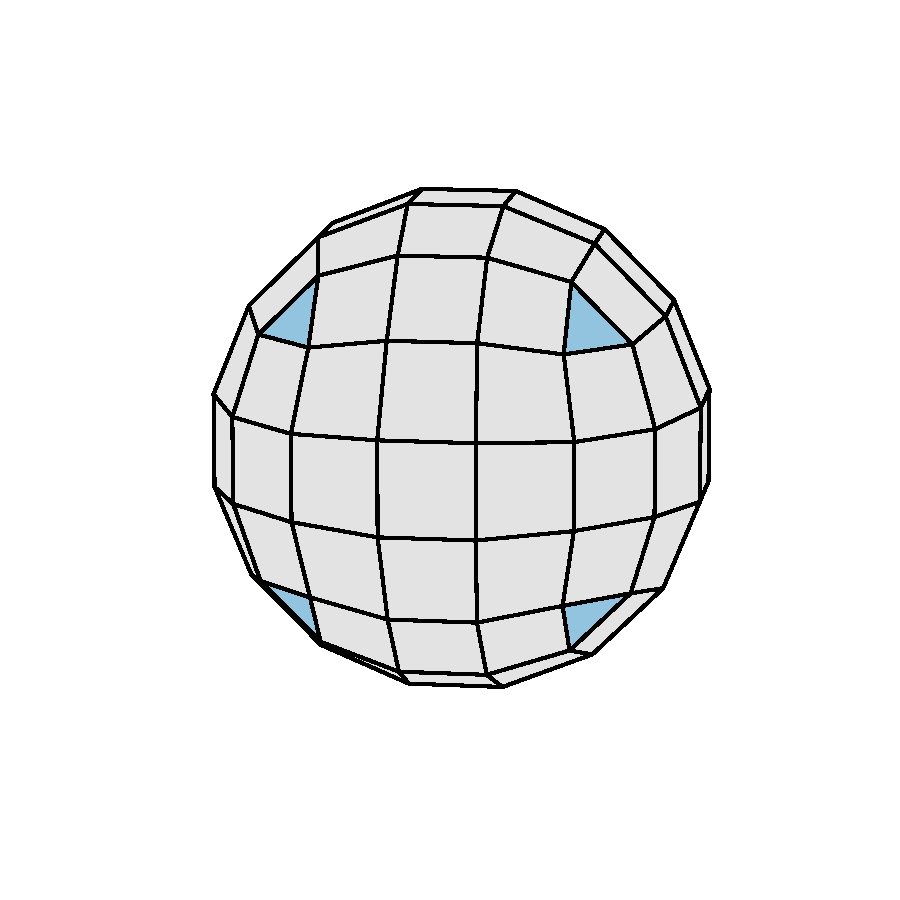
\includegraphics[height=2.4cm]{./figures/methods/full98.pdf}
         \caption{4\--coordinate fullerene.}
         \label{fig:latticesfull98}
     \end{subfigure}
     
     \caption{Panels (a)\--(c) give regular planar tilings of 6\--, 5\-- and 4\-- rings, where the ring size is related to the underlying atomic coordination. Panels (d) and (e) show the 3\-- and 4\-- coordinate tilings in spherical topology, where the mean ring size is reduced due to the change in the Euler characteristic.}
     \label{fig:lattices}
\end{figure}

\subsection{\lm's Law}

Knowing that the mean node degree is fixed by Euler's law, the next level of available information is the form of the underlying degree distribution, $p_k$.
Interestingly, the degree distributions found in physical ring networks seem relatively well defined.
For instance, it has been noted in models and realisations of \td{} silica glass that the ring statistics looked to follow a lognormal distribution \cite{Shackelford1981,Buchner2017}.
\lm{} \etal{} demonstrated that the distribution in 3-coordinate networks systems can be well described by a maximum entropy distribution \cite{Gervois1992}.
\lm's{} maximum entropy method is summarised here, trivially extended to arbitrary coordination.

The entropy of a probability distribution is defined as $S=-\sumk p_k\log p_k$. 
In addition, the degree distribution has the following constraints:
\begin{align}
		\sumk p_k &=1, \\
		\sumk kp_k&=\ki,  \label{con:lm2}\\
		\sumk \frac{p_k}{k}&=\text{constant} \label{con:lm3},
\end{align}
where the first two constraints correspond to the normalisation condition and the fixed mean ring size, and the final constraint will be discussed below.
The entropy can then be maximised using Lagrange's method of undetermined multipliers to yield the result:
\begin{equation}
	\label{eq:mepk}
	p_k = \frac{e^{-\lambda_1 k - \lambda_2 / k}}{\sumk e^{-\lambda_1 k - \lambda_2 / k}},
\end{equation}
which can be solved numerically by substitution into equations \eqref{con:lm2},\eqref{con:lm3}. 
By allowing the chosen constant to vary, a family of maximum entropy curves can be generated, as in figure \ref{fig:lm1}.
The resulting distributions can be summarised by relating the variance, $\mu_2=\kii-\ki^2$, to a single chosen node degree probability, leading to the plot known as \lm's law, given in figure \ref{fig:lm2}.
It is usually framed in the context of the proportion of hexagons in a system, $p_6$, for the precise reason that most networks have $\ki=6$ and $p_6$ as the largest contribution.
Many experimental and theoretical studies have shown good agreement to this law \cite{Caer1993,Cerisier1996,Miklius2012}.
Simple extensions of the classic law are however possible, by modifying the mean degree or the permitted degree range.
For instance, $k$ is usually taken in the interval $k\geq3$ (as the triangle, $k=3$, is the smallest polygon), but there can be manifestations of physical systems where only certain degrees are accessible \cite{Rivier1988}. \davidnote{Link to procrystal chapter}.
The resulting \lm{} curves for a selection of these modifications are given in figure \ref{fig:lm3}. 
\davidnote{explain these here or later?}
The maximum value of these curves can be simply determined by removing constraint \eqref{con:lm3}, equivalent to setting $\lambda_2=0$ in equation \eqref{eq:mepk}.
%Exploring these cases helps to understand the behaviour of \lm's law itself.
%By restricting the ring size to just $5\leq k \leq 7$ results in a straight line, which to satisfy Euler's law must have equation $\mu_2 = 1-p_6$.
%This line closely follows the high $p_6$ behaviour demonstrating that the initial deviation from the hexagonal lattice ($p_6=1$) is marked by the introduction of 5\-- and 7\-- ring defects.


\begin{figure}[h]
     \centering
     
     \begin{subfigure}[b]{0.45\textwidth}
         \centering
         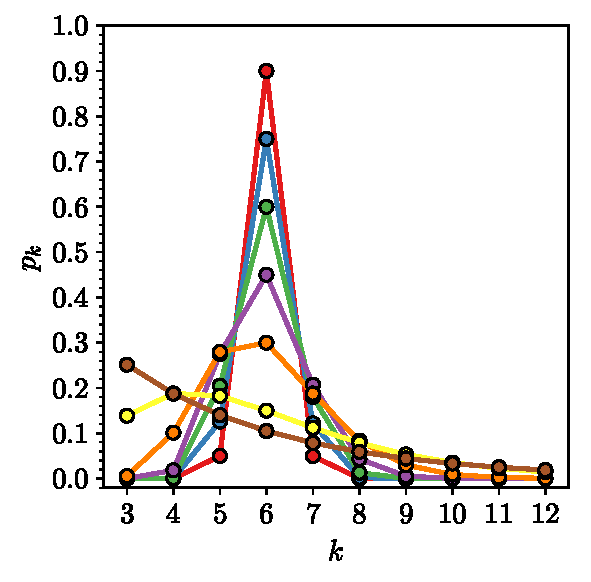
\includegraphics[width=\textwidth]{./figures/methods/lm_1.pdf}
         \caption{Maximum entropy distributions.}
         \label{fig:lm1}
     \end{subfigure}
     \hfill
      \begin{subfigure}[b]{0.45\textwidth}
         \centering
         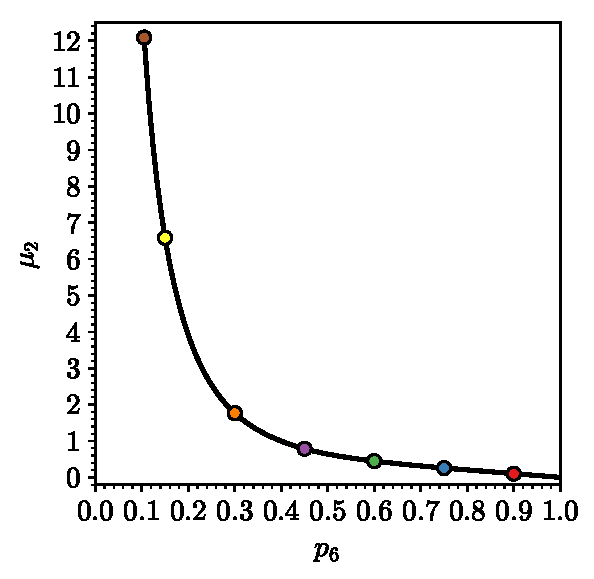
\includegraphics[width=\textwidth]{./figures/methods/lm_2.pdf}
         \caption{\lm's law.}
         \label{fig:lm2}
     \end{subfigure}
     \hfill
     
      \begin{subfigure}[b]{0.45\textwidth}
         \centering
         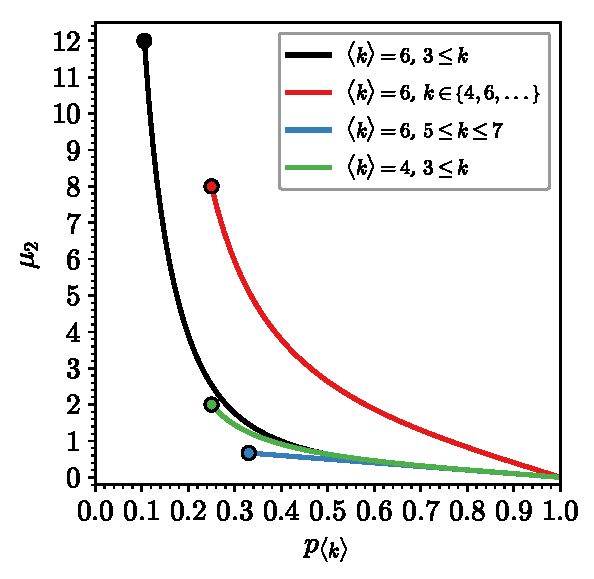
\includegraphics[width=\textwidth]{./figures/methods/lm_3.pdf}
         \caption{Extensions to \lm's law.}
         \label{fig:lm3}
     \end{subfigure}
     \hfill

    
     \caption{Illustration of \lm's maximum entropy method. Panel (a) gives examples of explicit maximum entropy distributions with different values of $p_6$. Panel (b) shows how these distributions can be summarised in a plot of $p_6$ \vs{} $\mu_2$ (\lm's law). Panel (c) provides extensions to the law by modifying the underlying constraints of the mean ring size and allowable $k$\--range.}
     \label{fig:lm}
\end{figure}

The only somewhat puzzling aspect of this successful theory is the choice of constraint \eqref{con:lm3}.
It was originally rationalised on the basis that the areas of rings of a given size, $A_k$, can be well fit by an expression $A_k = ak+b+c/k$, where $a$, $b$ and $c$ are constants.
As noted at the time, this is by no means true for all systems and in fact is contrary to the widely known Lewis law, which states that $A_k$ is linear in $k$ for many observable networks \cite{Lewis1928,Fortes1995,Kim2014}.
Despite this, the universality of the \lm{} law suggests that there must be a physical basis to \eqref{con:lm3}, and in the section \davidnote{Link to later networks} it will be demonstrated that it can be regenerated by considering ring adjacencies.

\subsection{\aw{} Law}

The ring statistics given by \lm's law are an important measure for physical networks, but they do not provide a complete characterisation of the ring structure, as they say nothing about the ring adjacencies. 
This is important because whilst with the same ring statistics it is theoretically possible to organise the rings in many different arrangements, it is well known experimentally that only a subsection of these are observed.
The vast majority of physical systems have a preference for small rings ($k<\ki$) be adjacent to large rings ($k>\ki$).
This effect was first noted in the grains of polycrystals by Aboav \cite{Aboav1970}.
Aboav quantified these ring correlations by measuring the mean ring size about a $k$\--ring, denoted $m_k$, and found empirically that $m_k \approx 5 + 8/k$.

In an attempt to explain this observation, Weaire came across the following relation
\begin{equation}
	\label{eq:weairesumrule}
	\sumk km_kp_k = \sumk k^2p_k = \mu_2 + \ki^2 \,,
\end{equation}
known as Weaire's sum rule \cite{Weaire1974}.
From this he suggested the modification of $m_k=5+\left(6+\mu_2\right)/k$ which satisfied this rule.
Aboav's original equation then became a special case when $\mu_2=2$, which is close to the expected value for a random collection of Voronoi polygons (see section \davidnote{link to Poisson\--Voronoi}).
Aboav then proposed that if a generic form of $m_k = A + B/k$ was used in conjunction with Weaire's sum rule then
\begin{equation}
	m_k = A+\frac{\mu_2+\ki^2-A\ki}{k}\,.
\end{equation}
This is now more commonly expressed in the linear form \cite{Chiu1995}:
\begin{equation}
	\label{eq:aboavweaire}
	km_k = \mu_2+\ki^2+\ki\left(1-\alpha\right)\left(k-\ki\right).
\end{equation}
Equation \ref{eq:aboavweaire} is known as the \aw{} law and relates the mean ring size about a given central ring to a single fitting parameter, $\alpha$.
The value of $\alpha$ describes the strength of the ring correlations, with a larger positive value indicating a greater tendency for small\--large ring adjacencies.
More specifically, the random limit can be deduced by evaluating $\frac{\partial{m_k}}{\partial{x}}=0$ as \cite{Delannay1994}:
\begin{equation}
	\label{eq:awrandlim}
	\alpha=-\frac{\mu_2}{\ki^2} \,.
\end{equation}
Hence all systems with $\alpha>-\mu_2/\ki^2$ have more small\--large ring  adjacencies than would be expected from chance whilst conversely those with $\alpha<-\mu_2/\ki^2$ have more small\--small and large\--large pairings.

\begin{figure}[tb]
     \centering
      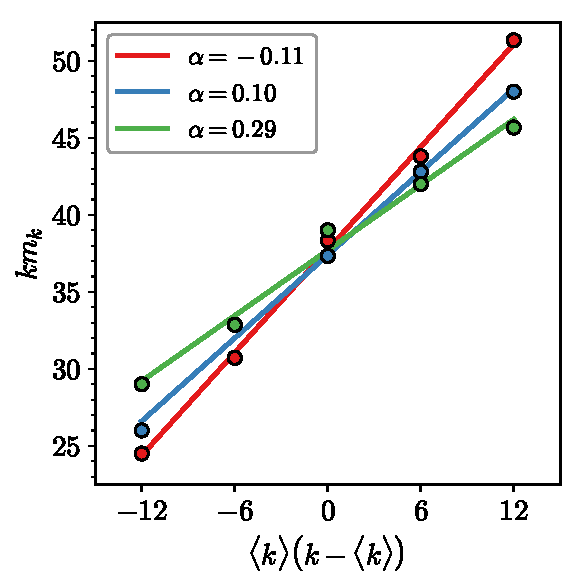
\includegraphics[width=8cm]{./figures/methods/aw_demo.pdf}
     \caption{Calculation of an \aw{} fit for three configurations (shown in figure \ref{fig:zach}(a)\--(c)). The value of the $\alpha$ parameter quantifies the tendency of small rings to be adjacent to large rings, with a larger value indicating stronger small\--large ring correlations.}
     \label{fig:awdemo}
\end{figure}

Despite the \aw{} law being purely empirical and there being no topological requirement for $m_k$ to vary systematically $k$, the law does seem to hold well for a diverse set of physical systems.
The law is well used for example in studies of materials, emulsions, biological tissues as well as in planetary science \cite{LeRoux2013,Roy2018,Noever1992,Mombach1993,Pedro2008}.
As an example of the calculation of the \aw{} parameter, the plots of the fits for the systems in figure \ref{fig:zach} are presented in figure \ref{fig:awdemo}, along with the corresponding $\alpha$ parameters.
This demonstrates two contrasting aspects of the \aw{} law. 
Firstly the law holds very well, especially given the fact that these samples consist of just twenty rings each.
However, it also demonstrates that the law is by no means exact and that some greyness is inevitably introduced during the linear regression.

\section{General \mc{} Methods}
\label{sec:mc}

\mc{} methods are a class of computational algorithms designed to solve complex problems stochastically.
These normally fall into the broad categories of calculating integrals, sampling probability distributions and finding global minima of very high dimensional functions \-- tasks which are often incredibly hard to compute deterministically.
Since their initial development in the mid\--20\th{} century, such methods have become an invaluable tool for solving problems in the physical sciences.
\mc{} methods are used in this context for calculating thermodynamic averages of properties in equilibrium systems; finding the minima in potential energy surfaces of small molecules, glasses, crystals and biomolecules; as well as non\--equilibrium simulations such as growth of crystals and thin\--films \cite{Landau2014,Wales1999,Levi1997,Ratsch2003,Kob1999,Jensen1999}.
In this thesis these \mc{} methods  will be used in a variety of contexts chapter xxx \davidnote{fill this in}.
Therefore, the general theory is presented here along with specific details of two established methods: bond switching and hard particle \mc{} given in the following section.

\subsection{Statistical Mechanics}

The total energy of a system with a fixed number of particles, $\mathcal{N}$, is given by the Hamiltonian,
\begin{equation}
	\ham = \ken+\pen \,,
\end{equation}
where $\ken$ is the kinetic energy as a function of all particle momenta and $\pen$ is the potential energy as a function of all particle positions \cite{Frenkel2002}.
The positions and momenta comprise the phase space of the system.
At fixed volume, $\mathcal{V}$, and temperature, $T$, all the the essential thermodynamic information is then provided through the classical canonical partition function:
\begin{equation}
	Q = \frac{1}{h^{D\mathcal{N}}\mathcal{N}!}\int \dd\mathbf{p}\,\dd\mathbf{r}\,\exp{\left[-\ham/ \kb T\right]}\,,
\end{equation}
where $D$ is the number of spatial dimensions.
This can be factorised into kinetic and potential components as
\begin{equation}
	Q = \frac{1}{h^{D\mathcal{N}}\mathcal{N}!}\int \dd\mathbf{p}\,\exp{\left[-\ken/\kb T\right]} \int \dd\mathbf{r}\,\exp{\left[-\pen/\kb T\right]} \,,
\end{equation}
where
\begin{equation}
	Z = \int \dd\mathbf{r}\,\exp{\left[-\pen/\kb T\right]}
\end{equation}
is the configurational integral \cite{Allen2017}. 
As will be shown, in \mc{} simulations it is the energetic differences between configurations that are required, and so at constant temperature the kinetic component can be neglected and it is only the configurational integral that is of importance.
In this case the probability density of the system being in the configuration $\mathbf{r}$ is given by the Boltzmann distribution:
\begin{equation}
	\label{eq:boltzmann}
	P\left(\mathbf{r}\right) = \frac{\exp{\left[-\pen/\kb T\right]}}{Z}\,.
\end{equation}
This allows the expectation value of an observable of the system, $\obs$, to be determined from:
\begin{equation}
	\label{eq:expectationobs}
	%\langle A \rangle = \frac{1}{Z}\int \dd\mathbf{r}\,\obs\exp{\left[-\pen/\kb T\right]} \,.
		\langle A \rangle = \int \dd\mathbf{r}\,\obs P\left(\mathbf{r}\right) \,.
\end{equation} 
The expectation value is then the ratio of two $\mathcal{N}D$ dimensional integrals.
The next section shows how these can be evaluated by \mc{} sampling.

\subsection{Importance Sampling}

An integral of form \eqref{eq:expectationobs} can be evaluated numerically by a number of methods.
As an illustration, consider the simple example of a \td{} potential energy surface in figure \ref{fig:montecarloint}.
To calculate the expectation value of the potential energy one must evaluate the integral
\begin{equation}
	\langle \mathcal{U} \rangle = \int_{0}^{L_y}\int_{0}^{L_x} \dd x \dd y\, \mathcal{U}\left(x,y\right)\mathcal{P}\left(x,y\right)\,.
\end{equation}
One way to achieve this would be to use standard numerical methods such as the trapezium rule or Simpson's rule to calculate the potential energy over a regular grid of points, as in figure \ref{fig:montecarloint1}, weighting each according to the Boltzmann distribution.

An alternative would be to take a stochastic approach.
In the simplest implementation, a series of $S$ random sampling points, $\left(x_i,y_i\right)$, can be generated uniformly in the intervals $\left[0,L_x\right]$ and $\left[0,L_y\right]$, as in figure \ref{fig:montecarloint2}.
Weighting these according to the Boltzmann distribution and averaging gives an estimation to the integral:
\begin{equation}
	\langle \mathcal{U} \rangle = \frac{L_xL_y}{S}\sum_{i=1}^{S} \mathcal{U}\left(x_i,y_i\right)\mathcal{P}\left(x_i,y_i\right)\,,
\end{equation}
which converges to the exact value as $S\rightarrow\infty$.

However, both quadrature and \mc{} uniform sampling suffer from the same inefficiency.
As can be seen in both schemes, many of the sampling points fall in regions of phase space where the potential energy is high and hence the weighting probability distribution is very small at reasonable temperatures.
In effect, significant effort is spent calculating regions where the contribution to the total integral is negligible.
A better approach is therefore to generate a series of $S$ random sampling points, $\left(x_i,y_i\right)$, according to the distribution $\mathcal{P}\left(x,y\right)$, as in figure \ref{fig:montecarloint2}.
The expectation value of the observable can then be calculated using a simple average:
\begin{equation}
	\langle \mathcal{U} \rangle = \frac{1}{S}\sum_{i=1}^{S} \mathcal{U}\left(x_i,y_i\right)\,.
\end{equation}
This is known as importance sampling and is vastly more efficient when dealing with an aggressive probability distribution like the Boltzmann, where only a small proportion of the phase space is accessible.

Whilst this scheme is ideal theoretically, it is impracticable for physical systems.
This is because for any problem of real interest one lives in a ``black box'' where the functional form of the potential energy surface in its hundreds if not thousands of dimensions is unknown.
In this case often the only way of learning about the form is by on\--the\--fly exploration of the surface \cite{Brooks2011}.
This can be achieved by talking a random walk through configurational space using Markov chain \mc.

\begin{figure}[h]
     \centering
     
     \begin{subfigure}[b]{0.45\textwidth}
         \centering
         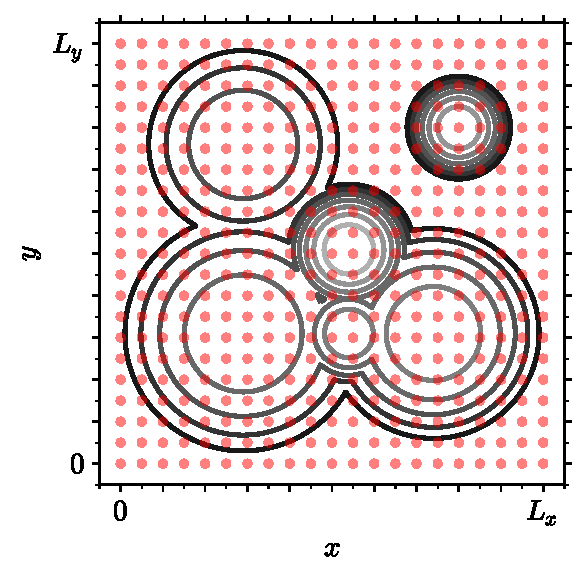
\includegraphics[width=\textwidth]{./figures/methods/mc_2d_quad.pdf}
         \caption{Quadrature.}
         \label{fig:montecarloint1}
     \end{subfigure}
     \hfill
     \begin{subfigure}[b]{0.45\textwidth}
         \centering
         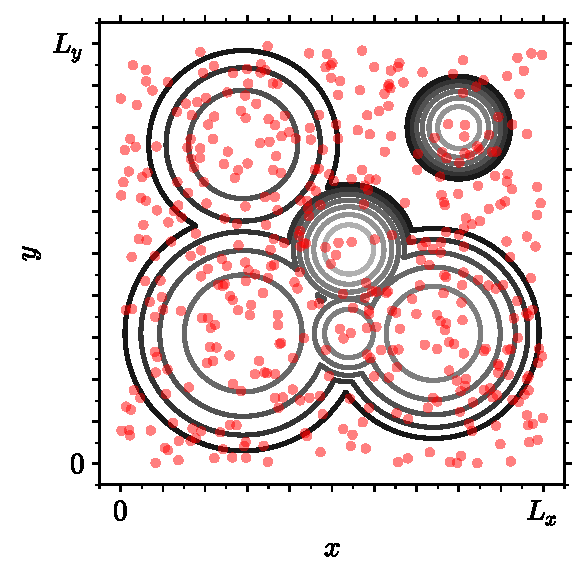
\includegraphics[width=\textwidth]{./figures/methods/mc_2d_rand.pdf}
         \caption{Uniform Sampling.}
         \label{fig:montecarloint2}
     \end{subfigure}
     \hfill
     
     \begin{subfigure}[b]{0.45\textwidth}
         \centering
         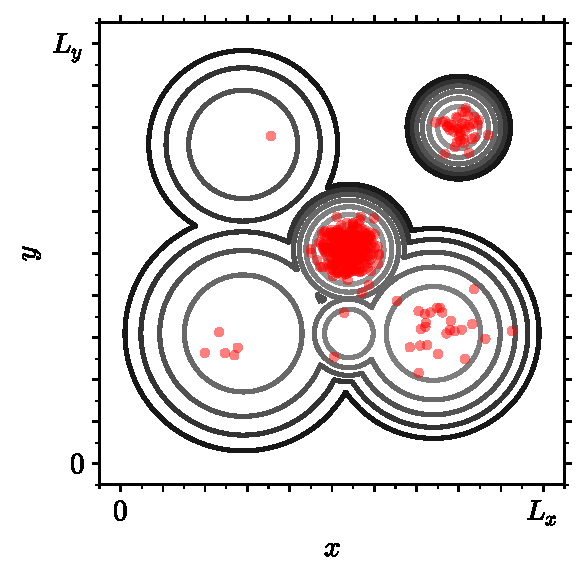
\includegraphics[width=\textwidth]{./figures/methods/mc_2d_imp.pdf}
         \caption{Importance Sampling.}
         \label{fig:montecarloint3}
     \end{subfigure}
     \hfill
     \begin{subfigure}[b]{0.45\textwidth}
         \centering
         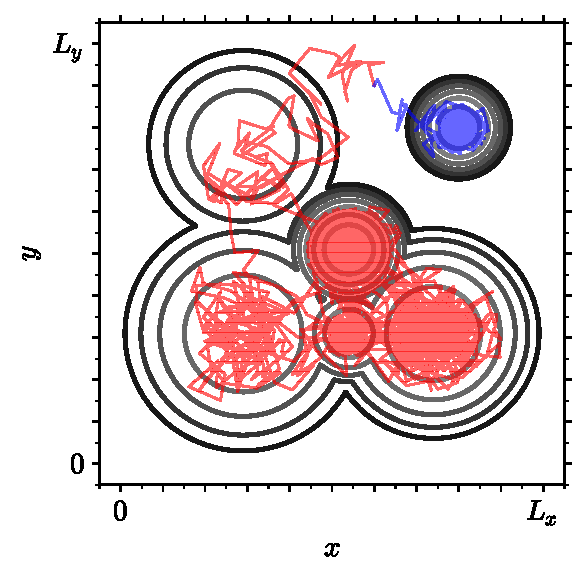
\includegraphics[width=\textwidth]{./figures/methods/mc_2d_mcmc.pdf}
         \caption{Markov Chain \mc}
         \label{fig:montecarloint4}
     \end{subfigure}
     \hfill
    
     \caption{Demonstration of different sampling methods with an example \td{} potential energy surface (contour lines). Panels(a)\--(c) display the same number of (red) sampling points. Panel (a) shows conventional quadrature where the surface is divided into a regular grid of sampling points which are then weighted by the Boltzmann distribution. Panel (b) shows \mc{} sampling with a uniform distribution of points which again must be Boltzmann\--weighted. Panel (c) shows \mc{} importance sampling with points now selected according to the Boltzmann distribution. Panel (d) shows Markov chain \mc{} with two random walks through phase space (red and blue lines) starting from different random seeds.}
     \label{fig:montecarloint}
\end{figure}

\subsection{Markov Chain Monte Carlo}

Markov chain Monte Carlo provides a framework to perform importance sampling on a potential energy surface.
A system of interest can exist in a (very large) number of configurational states, $\left\{\mathbf{r}_0,\mathbf{r}_1,\dots,\mathbf{r}_M\right\}$.
A Markov chain can then be constructed from this set, whereby a sequence of states is generated stochastically across a series of steps, $s=0,1,\dots,S$.
In this process, the probability of moving between states at each step is given by the transition matrix, $\bm{\pi}$, where each element, $\pi_{ij}$, gives the probability of moving from the state $\mathbf{r}_i$ to another state $\mathbf{r}_j$.  
This leads to the two relationships:
\begin{align}
	0\leq \pi_{ij} &\leq 1\,, \\
	\sum_{j} \pi_{ij} &= 1\,, \label{eq:tmrowsum}
\end{align}
the first being a statement of the probabilistic nature of the elements whilst the second ensures all transfer remains within the state space \cite{Frenkel2002,Allen2017,Brooks2011}.

The probability that the system is in each state at a given step, $s$, can be represented by the row vector $\mathbf{P}_s$.
This probability distribution evolves with each step as $\mathbf{P}_{s+1}=\mathbf{P}_{s}\bm{\pi}$, so that starting from any initial distribution, $\mathbf{P}_0$, it follows that $\mathbf{P}_S=\mathbf{P}_0\bm{\pi}^S$. 
The question is then as to the behaviour as $S\rightarrow \infty$.
Provided certain criteria are met, the distribution will tend to a stationary distribution, $\mathbf{P}$, which satisfies the eigenvalue equation 
\begin{equation}
	\mathbf{P} = \mathbf{P}\bm{\pi}\,, \label{eq:mcmceig}
\end{equation}
regardless of the initial distribution (although the speed of the convergence does depend on $\mathbf{P}_0$).
This will occur only if the system is \textit{ergodic}, meaning that every state is connected to every other by some finite path.

In a discrete analogue to equation \eqref{eq:expectationobs}, the expectation value of an observable, $A$, can be calculated from the ensemble average:
\begin{equation}
	\langle A \rangle = \sum_{i=1}^{M} A\left(\mathbf{r}_i\right)\mathcal{P}\left(\mathbf{r}_i\right)\,,
\end{equation}
where $\mathcal{P}\left(\mathbf{r}_i\right)$ are the elements of $\mathbf{P}$.
However, as previously mentioned the number of discrete states is usually exceedingly large and so calculating the average over all states is not possible.
The solution is to take a random walk across through configurational space, sampling explicit states to form the chain $X_0,X_1,\dots,X_S$; where each move is chosen randomly according to the transition matrix $\bm{\pi}$.
In this case the expectation of the same observable can be calculated from the average over the sampled states:
\begin{equation}
	\langle A \rangle = \frac{1}{S}\sum_{i=1}^{S} A\left(X_i\right)\,,
\end{equation}
where the true value is approached as $S\rightarrow \infty$.

In this section the problem of sampling phase space efficiently has been reformulated, but as yet not solved. 
This is because the form of the transition matrix is still unknown.
Instead only the ideal form of the limiting probability distribution, $\mathbf{P}$, is available \-- where the elements follow the Boltzmann probabilities in equation \eqref{eq:boltzmann}.
A practical solution to this problem is provided by the Metropolis algorithm.

\subsection{Metropolis Algorithm}
\label{ssec:metropolis}

The Metropolis algorithm gives a prescription of how to construct a transition matrix, $\bm{\pi}$, with the requisite properties that samples the Boltzmann distribution \cite{Metropolis1953}.
Firstly, combining equations \eqref{eq:tmrowsum} and \eqref{eq:mcmceig} gives a condition on the transition matrix known as global balance:
\begin{equation}
	\sum_j \mathcal{P}\left(\mathbf{r}_i\right)\pi_{ij} = \sum_j \mathcal{P}\left(\mathbf{r}_j\right)\pi_{ji}\,.
\end{equation} 
Whilst it is possible to construct transition matrices which satisfy only global balance \cite{Manousiouthakis1999,Suwa2010,Michel2014}, it is practically simpler to satisfy global balance by applying the stronger condition of detailed balance:
\begin{equation}
	\mathcal{P}\left(\mathbf{r}_i\right)\pi_{ij} = \mathcal{P}\left(\mathbf{r}_j\right)\pi_{ji}\,.
\end{equation}
In the Metropolis algorithm the off\--diagonal elements of the transition matrix are written as the product of two probabilities: 
\begin{equation}
	\pi_{ij} = \begin{cases} 
		\tau_{ij}P_{ij} \quad & i\neq j \\
		1-\sum\limits_{j\neq i}\tau_{ij}P_{ij} \quad & i=j
	\end{cases}\,,
\end{equation}
where $\tau_{ij}$ is the trial probability of moving from state $\mathbf{r}_i$ to $\mathbf{r}_j$ and $P_{ij}$ is the probability of accepting the trial move.
To conform to detailed balance, the trial probabilities must be chosen to satisfy $\tau_{ij}=\tau_{ji}$.
Then, in the crux of the algorithm, the acceptance probabilities are given by
\begin{align}
	 P_{ij}&=\begin{cases}
	 	1 \quad &\mathcal{P}\left(\mathbf{r}_j\right)\geq \mathcal{P}\left(\mathbf{r}_i\right) \\
	 	\frac{\mathcal{P}\left(\mathbf{r}_j\right)}{\mathcal{P}\left(\mathbf{r}_i\right)} \quad & \mathcal{P}\left(\mathbf{r}_j\right)< \mathcal{P}\left(\mathbf{r}_i\right)
	 \end{cases}
	 =\begin{cases}
	 	1 \quad &\mathcal{U}\left(\mathbf{r}_j\right)\leq \mathcal{U}\left(\mathbf{r}_i\right) \\
	 	\frac{\exp\left[-\mathcal{U}\left(\mathbf{r}_j\right)/\kb T\right]}{\exp\left[-\mathcal{U}\left(\mathbf{r}_i\right)/\kb T\right]} \quad & \mathcal{U}\left(\mathbf{r}_j\right)>\mathcal{U}\left(\mathbf{r}_i\right)
	 \end{cases}\,,
\end{align}
which can be expressed more succinctly as
\begin{equation}
	\label{eq:metropolis}
	 P_{ij}=\text{min}\big[1,\exp\left[-\Delta \mathcal{U}/\kb T\right]\big]\,,
\end{equation}
where $\Delta \mathcal{U}$ is the difference in potential energy between the final and initial states.
The elegance of the Metropolis algorithm lies in the fact that the acceptance probability depends only on the ratio of the configuration probabilities removing the need for a normalising factor.
This means the relative probabilities can be used (which are computable) instead of the absolute probabilities (which are unknowable).

The final stage is the choice of the matrix of trial probabilities, $\bm{\tau}$. 
This is very flexible and one can be creative in the selection of trial moves, providing that the underlying matrix is symmetric and ergodic.
An effective strategy is to choose moves in which the trial state is relatively close to the current state to trace the paths of high probability in the system.
A summary of the Metropolis algorithm is therefore as follows:
\begin{enumerate}
	\item Initialise the system in a state $X_{s=0}$ and calculate the potential energy $\mathcal{U}\left(X_s\right)$
	\item Generate a trial state $X_t$ (a perturbation of $X_s$) according to $\tau_{st}$
	\item Calculate the potential energy of the trial state $\mathcal{U}\left(X_t\right)$
	\item Determine acceptance or rejection of the trial move according to the Metropolis criterion \eqref{eq:metropolis}
	\item Update the system to the new state: if the trial move is accepted $X_{s+1}=X_{t}$ otherwise $X_{s+1}=X_{s}$
	\item Repeat steps 2\--5
\end{enumerate}
There are a few practical factors related to the scheme above.
In Markov chain \mc{} it was previously mentioned that it takes time for the system to evolve to the stationary distribution.
Therefore it is necessary to have an equilibration period where the chain is generated but not used for sampling of observables.
In addition, whilst selecting trial moves close to the current state increases efficiency, it introduces correlation into the procedure.
A way around this is to not calculate observables based on every step, but rather after a number of statistically significant steps.

As an example of the Metropolis algorithm, consider again the \td{} potential energy surface in figure \ref{fig:montecarloint4}.
Here two simulation paths are displayed in red and blue, starting from the same initial state but with different starting points in the random number generators \ie{} random seeds.
As can be seen the Metropolis algorithm takes a random walk over the configurational space, conducting importance sampling as in \ref{fig:montecarloint3}.
However, in this example highlights a potential problem.
There are two regions of phase space with non\--zero probabilities which are separated by a relatively large energy barrier.
Although they are in principle linked by a path, the barrier may effectively mean they are disconnected on a reasonable simulation time scale, breaking ergodicity.
This manifests as the red walk sampling one region and the blue walk being trapped in the other region.
Using multiple seeds in this way helps to identify if any such behaviour is present.
If it leads to significant differences in the computed averages, more advanced techniques using enhanced sampling may have to be employed \cite{Torrie1977,Earl2005}.

\subsection{Global Optimisation \& Simulated Annealing}

So far in this section it has been shown how Monte Carlo methods can be used perform importance sampling of potential energy surfaces.
These methods can also be used to solve the related problem of finding global minima in potential energy surfaces and other more general functions.
Consider the case where there is an objective function, $\obj\left(\mathbf{r}\right)$, which depends on particle positions.
If it is known that there exists a solution where $\obj\left(\mathbf{r}\right)=0$, it may be sufficient to perform a standard random walk of the type in figure \ref{fig:montecarloint4} until a solution is found, using the more general Metropolis criterion:
\begin{equation}
	\label{eq:objmetropolis}
	P_{ij} = \min\big[1,\exp\left[-\Delta\Omega/\kb T\right]\big].
\end{equation}
There is of course a chance that the optimisation will not converge to the global minimum, most likely getting trapped in a local minimum (as for instance the blue path in \ref{fig:montecarloint4}).
One solution to this problem is just to keep restarting the algorithm with different initial conditions until the global minimum is obtained.

Often however the value of the global minimum is not known, as is the case for a potential energy surface, and this rudimentary approach is insufficient.
One must then employ a more sophisticated technique to find the global minimum of a very high dimensional and potentially rough surface.
This in itself is an extensive area of study and there are many approaches such as using genetic algorithms or basin\--hopping \cite{Hartke1993,Niesse1996,Wales1997}.
This thesis will use simulated annealing, which can be considered an extension to Metropolis \mc{} \cite{Kirkpatrick1983}.
In addition simulated annealing is effective for searching surfaces with many similar minima as in glasses \-- the name reflecting its origins in the analogous process in metallurgy to generate defect free metals.

\begin{figure}[tb]
     \centering
    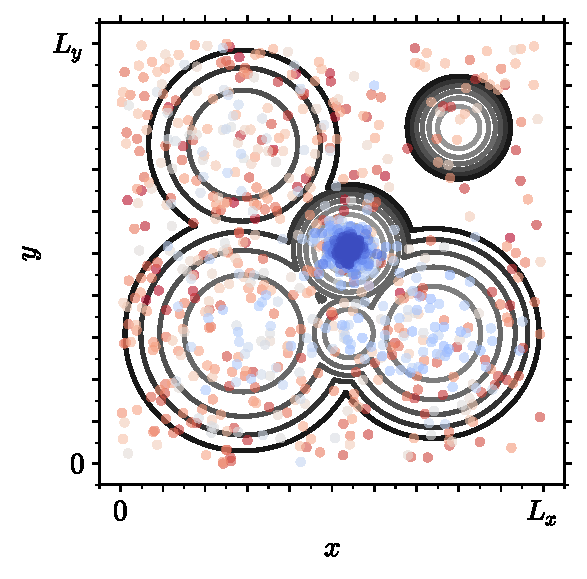
\includegraphics[width=0.45\textwidth]{./figures/methods/mc_2d_sa.pdf}
      \caption{Demonstration of the simulated annealing algorithm on a \td{} potential energy surface, with states coloured by temperature (red$\rightarrow$blue indicating hot$\rightarrow$cold. As the temperature is reduced the state converges on the global minimum.}
      \label{fig:montecarloint5}
\end{figure}

The simulated annealing algorithm proceeds as follows.
The system of interest is first thermalised by performing Metropolis \mc{} at infinite temperature \ie{} accepting every move. 
The system is then gradually cooled to zero temperature, with the Metropolis criterion \eqref{eq:objmetropolis} reducing the proportion of accepted moves.
In theory if the cooling is infinitely slow, the system is maintained in thermal equilibrium and will eventually reach the global minimum \cite{Henderson2003}.
In practice this is not realisable and so a cooling rate must be empirically selected.
Still it is possible for trapping to occur in local minima, especially if the transition between low energy states is very slow.
As before, one can then cycle the simulated annealing, repeatedly heating and cooling the system until the global minimum is found.
The simulated annealing algorithm is demonstrated with the \td{} potential energy surface in figure \ref{fig:montecarloint5}.
As can be seen at high temperature the entire surface is sampled, overcoming all energy barriers, but as cooling takes place the system settles into the low energy regions of the surface, finally terminating in the global minimum.

\section{Hard Particle \mc}

Hard particle Monte Carlo is one of the most well\--established computational methods in statistical physics.
Through its simplicity it is able to provide insight into the fundamental behaviour of particle systems and simulations of increasing size are still performed this century \cite{Isobe2016,Bernard2009,Anderson2013,Isobe2015}.
In this thesis it will be used to generate ring systems in the form of Voronoi tessellations (see sec \davidnote{link to voronoi}), in analogy to experimental colloidal systems \cite{Thorneywork2017}.

\subsection{Hard Particle Model}

Hard particle models are applicable over a range of dimensions.
In two dimensions the system consists of an arrangement of hard disks and in three dimensions hard spheres.
One can also take a quasi \td{} system, which comprises hard spheres confined to a plane.
Regardless of the dimensionality, the central principle is that no two particles in the system can have any degree overlap.
Formally, if the particle radii are denoted by $R_i$ and the distance between any pair of particle centroids by $d_{ij}$, the pair potential is:
\begin{equation}
	\mathcal{U}_{ij} = \begin{cases}
	\infty \quad &d_{ij}<R_i+R_j \\
	0 \quad &d_{ij}\geq R_i+R_j 
	\end{cases} \,.
\end{equation}
As the total energy is simply then
\begin{equation}
	\mathcal{U} = \sum_{i<j} \mathcal{U}_{ij}\,,
\end{equation}
it follows that if any pair of particles have overlap the system energy is infinite and the Boltzmann weighting is zero.

\subsection{\mc{} Simulation} 

Hard particle systems can be simulated using the Metropolis algorithm outlined in section \ref{ssec:metropolis}.
The system is initialised by selecting a random non\--overlapping configuration.
This can be achieved easily for low to medium densities by a greedy algorithm like random sequential addition, where particles are added successively in a manner which does not overlap with any previous particles \cite{Widom1966}.
For higher packing fractions a more sophisticated algorithm is needed \davidnote{Find refs}.

Once the initial configuration has been generated, it is evolved via two \mc{} moves.
The first is the displacement move, whereby a random particle is selected and translated according to a random vector with elements generated uniformly in the range $\left[-\delta,\delta\right]$.
If the displacement introduces any particle overlaps it is rejected, otherwise the system is updated to the new configuration, as illustrated in figure \ref{fig:hardmc1}\--\ref{fig:hardmc3}.
The value of $\delta$ is chosen for each simulation such that the proportion of accepted moves is $\sim 50\%$, allowing for efficient searching of configurational space.
The optimal value can be determined by continuous adjustment during equilibration.

The second is the swap move, where two random particles are selected their radii exchanged \cite{Grigera2001,Ninarello2017}. 
Once again a swap move is only accepted if it does not lead to any overlapping particles and is demonstrated in figure \ref{fig:hardmc4}\--\ref{fig:hardmc6}.
The swap move is used to increase the efficiency in simulations of polydisperse particles and is an example of how the design of \mc{} moves can be flexible and they do not have to have a direct physical basis. 
The swap move is attempted for every ten displacement moves. 

\begin{figure}[bt]
     \centering
     
     \begin{subfigure}[b]{0.25\textwidth}
         \centering
         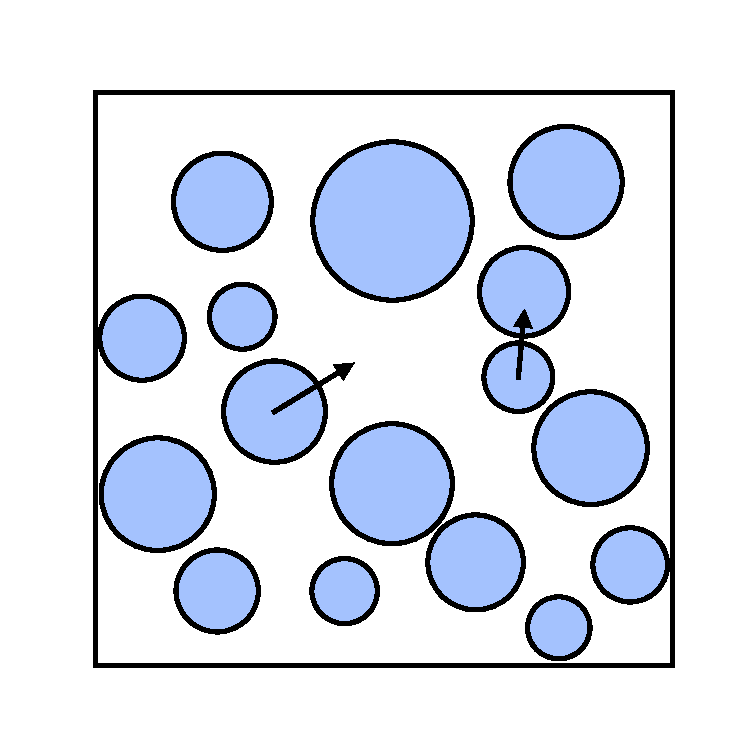
\includegraphics[width=\textwidth]{./figures/methods/mc_move_a.pdf}
         \caption{}
         \label{fig:hardmc1}
     \end{subfigure}
     \hfill
     \begin{subfigure}[b]{0.25\textwidth}
         \centering
         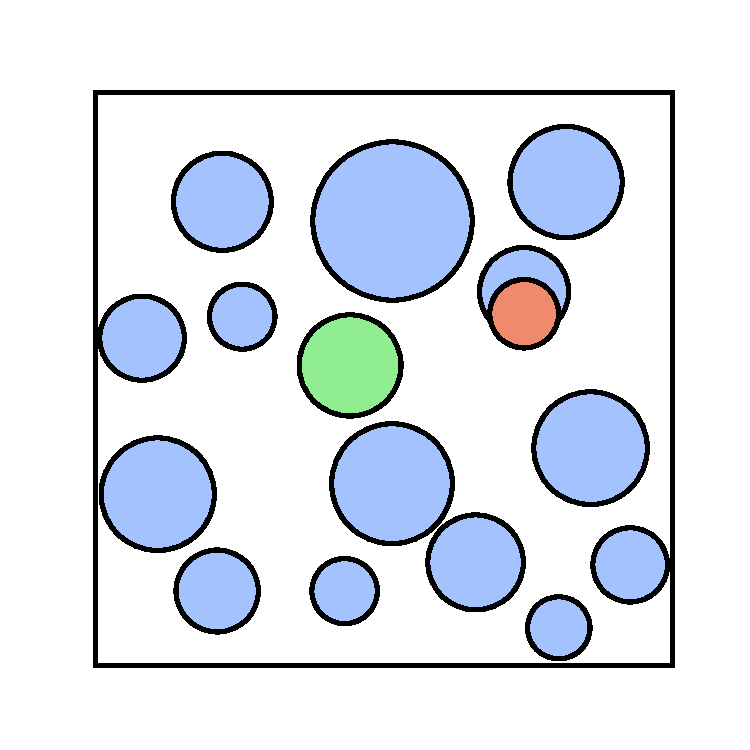
\includegraphics[width=\textwidth]{./figures/methods/mc_move_b.pdf}
         \caption{}
         \label{fig:hardmc2}
     \end{subfigure}
     \hfill
     \begin{subfigure}[b]{0.25\textwidth}
         \centering
         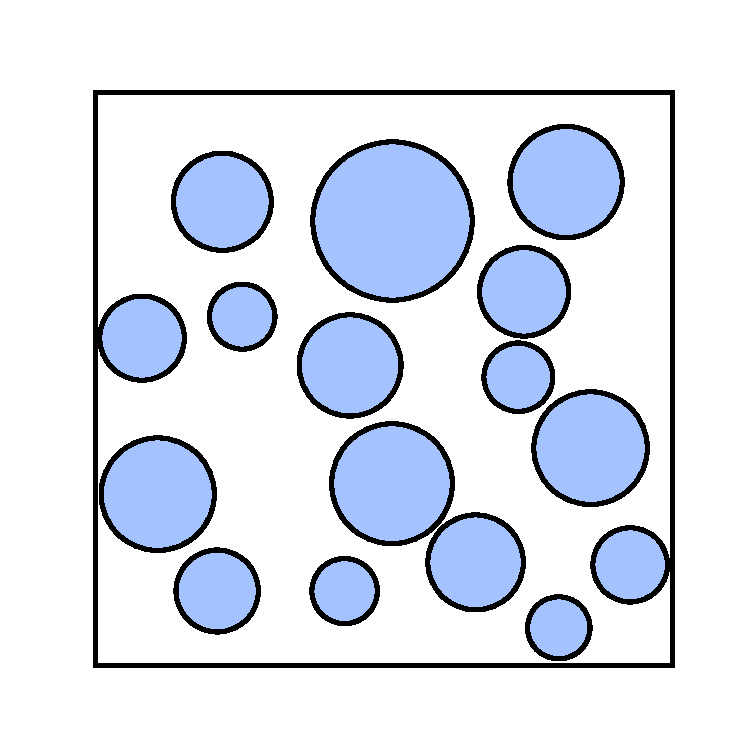
\includegraphics[width=\textwidth]{./figures/methods/mc_move_c.pdf}
         \caption{}
         \label{fig:hardmc3}
     \end{subfigure}
     \hfill
     
       \begin{subfigure}[b]{0.25\textwidth}
         \centering
         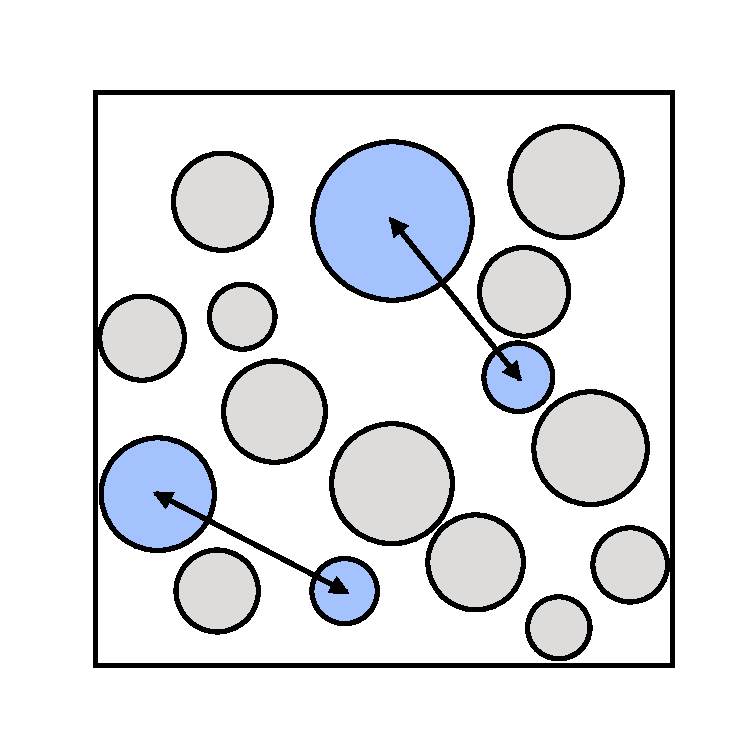
\includegraphics[width=\textwidth]{./figures/methods/mc_move_d.pdf}
         \caption{}
         \label{fig:hardmc4}
     \end{subfigure}
     \hfill
     \begin{subfigure}[b]{0.25\textwidth}
         \centering
         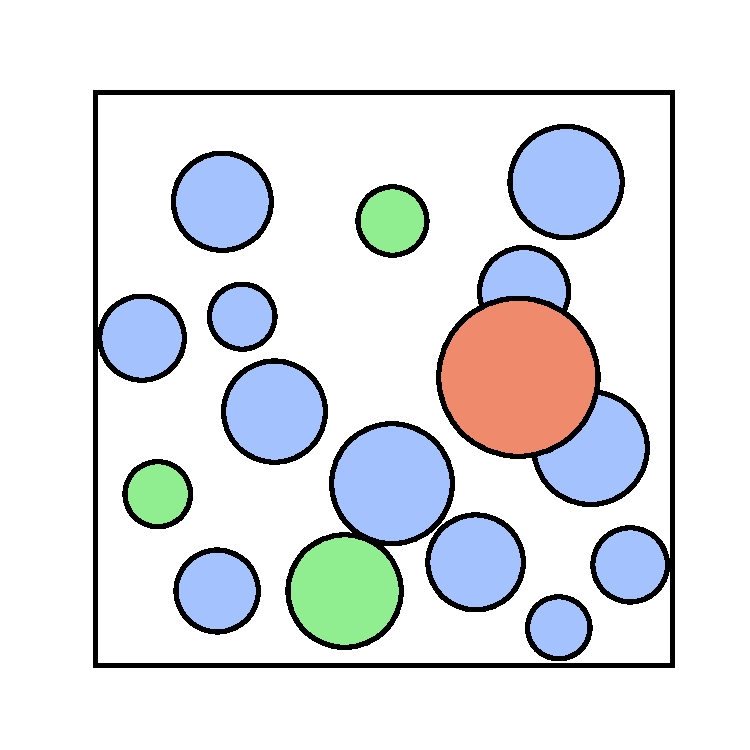
\includegraphics[width=\textwidth]{./figures/methods/mc_move_e.pdf}
         \caption{}
         \label{fig:hardmc5}
     \end{subfigure}
     \hfill
     \begin{subfigure}[b]{0.25\textwidth}
         \centering
         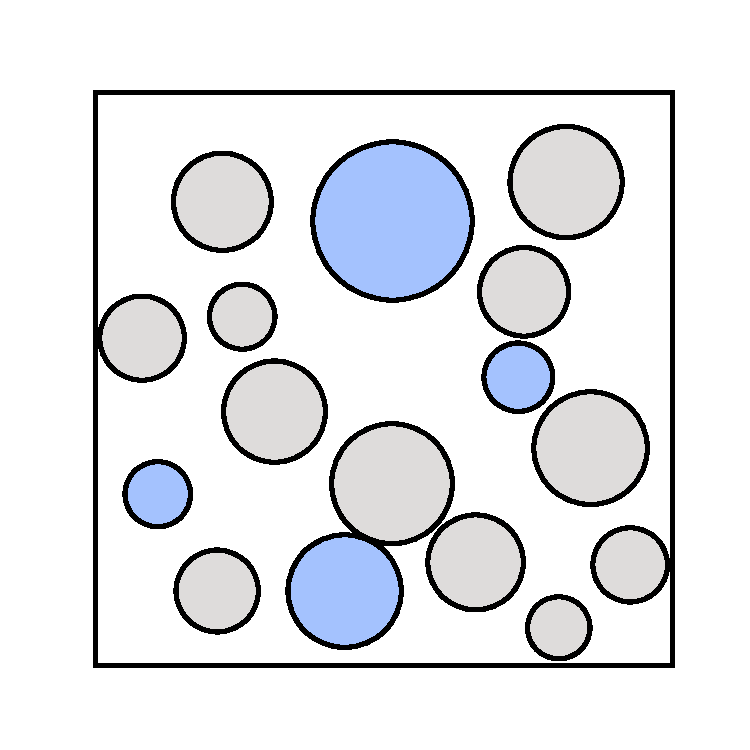
\includegraphics[width=\textwidth]{./figures/methods/mc_move_f.pdf}
         \caption{}
         \label{fig:hardmc6}
     \end{subfigure}
     \hfill
   
     \caption{Demonstration of two displacement (a)\--(c) and two swap (d)\--(f) moves in hard particle \mc.
     In displacement moves, particles are randomly selected and assigned a trial random displacement vector (a). In swap moves, two particles are randomly selected and their radii trial swapped (b). The trial move is then examined to see if it introduces any particle overlaps (b),(e). If there are no overlaps (green), then the trial move is accepted and the system updated but otherwise (red) the move is rejected and the system returns to the previous state (c),(f).
     }
     \label{fig:hardmc}
\end{figure}

\begin{figure}[tb]
	\centering
	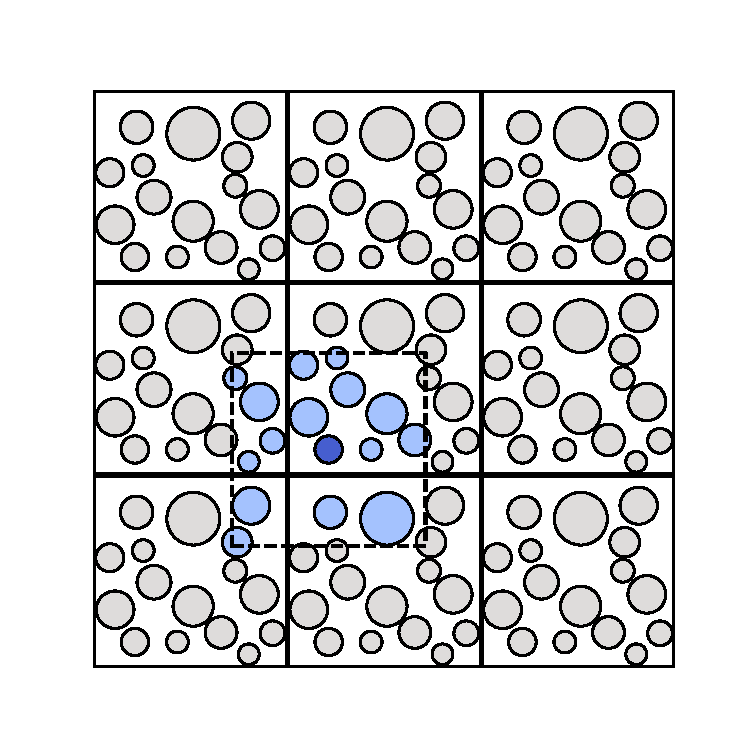
\includegraphics[width=8cm]{./figures/methods/mc_move_g.pdf}
	\caption{Simulation of bulk system is achieved using periodic boundary conditions, where a central cell is surrounded by repeated images of itself. A particle of interest (dark blue) then interacts with the nearest images of every other particle (light blue).}
	\label{fig:pbc}
\end{figure}

Finally, to remove the presence of an interface in the system, simulation is performed with periodic boundary conditions.
In this scheme the central simulation cell is repeated to form an infinite lattice, so that every particle experiences a bulk environment.
Coupled with this is the use of the minimum image convention, where each particle then only interacts with the nearest repeated image of all the remaining particles.
This is illustrated in figure \ref{fig:pbc}. 